\chapter{Architettura dell'ontologia}
In questo capitolo illustreremo più in dettaglio la struttura e le scelte progettuali adottate per la creazione di Motology, partendo dalle classi, proprietà e data properties utilizzate, terminando con le regole SWRL.

\section{Specifiche dell'ontologia}
\begin{figure}[H]
    \begin{center}
        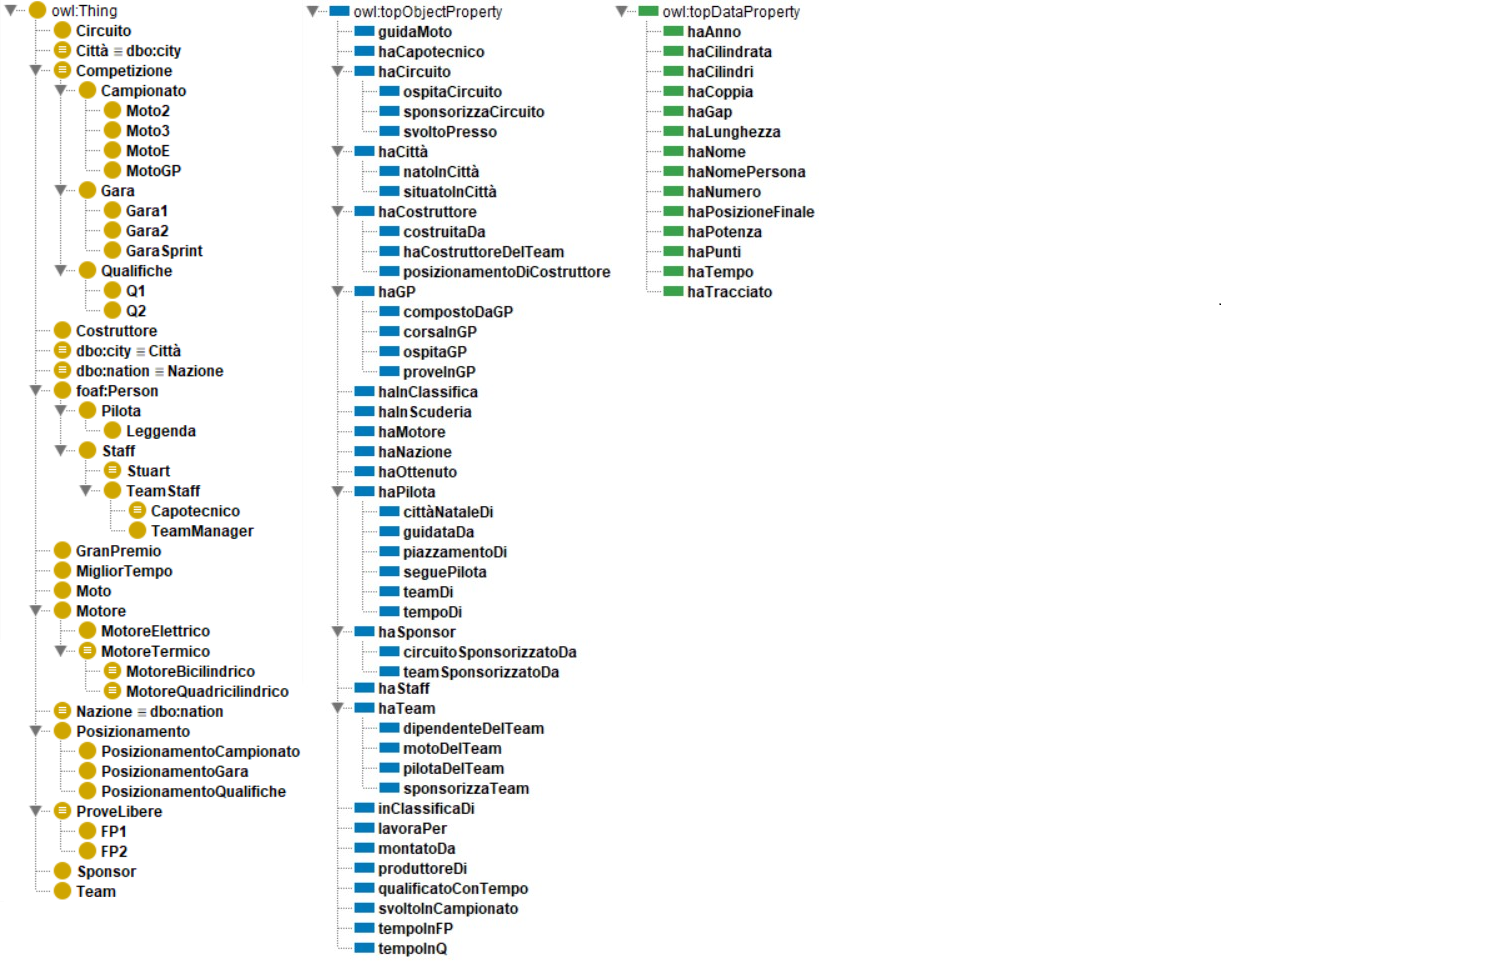
\includegraphics[scale=0.83]{img/Gerarchie.png}
       \caption{Totalità delle Classi, Object Properties e Data Properties.} 
    \end{center}
\end{figure}

\subsection{Classi}
Dopo la panoramica nel capitolo precedente dove sono state spiegte le classi principali, scenderemo più nel dettaglio riportando una spiegazione sintetica per ognuna della 44 classi che formano Motology.

\begin{itemize}
  \item \textbf{Città}: Rappresenta una città, come "insediamento umano di grandi dimensioni" (DBPedia).
  \item \textbf{Nazione}: Rappresenta una nazione, "comunità stabile di persone" (DBPedia).
  \item \textbf{Competizione}: Rappresenta un qualunque evento competitivo che vede come risultato una classifica, ha come sottoclassi Campionato, Gara e Sessione di Qualifica.
  \item \textbf{Campionato}: Rappresenta un campionato, a sua volta suddiviso in "classi" contraddistinte dalle caratteristiche delle moto che vi partecipano (es. Campionato di Moto2).
  \item \textbf{Moto2}: Rappresenta il campionato Moto2, contraddistinto da motori fino a 765 cm³ a quattro tempi fornito a tutte le squadre dalla stessa casa costruttrice.
  \item \textbf{Moto3}: Rappresenta il campionato Moto2, contraddistinto da motori fino a 250 cm³ a quattro tempi monocilindrici.  
  \item \textbf{MotoE}: Rappresenta il campionato MotoE, contraddistinto da prototipi a motore elettrico e alimentazione a batteria, il campionato più giovane nato nel 2019.
  \item \textbf{MotoGP}: Rappresenta il campionato MotoGP, contraddistinto da motori fino a 1000 cm³ a quattro tempi. \\ Per ogni campionato negli scorsi anni sono cambiate numerose volte le specifiche delle moto, inoltre negli anni anche i campionati sono notevolmente cambiati (seguendo il progresso tecnologico e l'attenzione all'ambiente). Motology per come è strutturata permette di modellare agilmente questi cambiamenti nel tempo.
  \item \textbf{Gara}: Rappresenta una singola gara di uno specifico campionato in uno specifico gran premio.
  \item \textbf{Gara1}: Nel caso di alcuni specifici campionati che la prevedono, rappresenta la prima gara di un Gran Premio.
  \item \textbf{Gara2}: Nel caso di alcuni specifici campionati che la prevedono, rappresenta la seconda gara di un Gran Premio
  \item \textbf{GaraSprint}: Nel caso di alcuni specifici campionati che la prevedono, rappresenta una gara speciale di un Gran Premio contraddistinta da meno giri.
  \item \textbf{Qualifiche}: Rappresenta una sessione di qualifica, competizione che permette di determinare le posizioni di partenza per una gara.
  \item \textbf{Q1}: Rappresenta la prima sessione di qualifica.
  \item \textbf{Q2}: Rappresenta la seconda sessione di qualifica.
  \item \textbf{Circuito}: Rappresenta una pista chiusa adibita a gare (anche di natura differente da quelle del motomondiale).
  \item \textbf{Costruttore}: Rappresenta il brand di un'azienda che costruisce prototipi da corsa.
  \item \textbf{ProveLibere}: Rappresenta le sessioni di prove libere prima di una gara.
  \item \textbf{FP1}: Rappresenta la prima sessione di prove libere.
  \item \textbf{FP2}: Rappresenta la seconda sessione di prove libere.
  \item \textbf{GranPremio}: Rappresenta un Gran Premio, evento cardine del motomondiale che contraddistingue tutte le competizioni che avverranno in uno specifico circuito (uno per stato, per questo diremo "Gran Premio d'Italia per indicare l'insieme delle competizioni svolte nel circuito del Mugello).
  \item \textbf{MigliorTempo}: Rappresenta il miglior tempo registrato da un partecipante in una competizione o in una prova libera.
  \item \textbf{Moto}: Rappresenta un prototipo da gara di un motociclo, veicolo a motore dotato di due ruote.
  \item \textbf{Motore}: Rappresenta un propulsore.
  \item \textbf{MotoreElettrico}: Rappresenta un motore elettrico (con caratteristiche legate ad emissioni e alimentazione molto differenti da motori termici).
  \item \textbf{MotoreTermico}: Rappresenta un motore a combustione interna.
   \begin{figure}[H]
    \begin{center}
        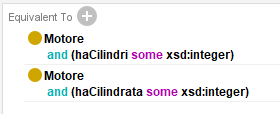
\includegraphics[scale=1]{img/spec_motoretermico.png}
       \caption{Modellazione motore termico.} 
    \end{center}
\end{figure}
  \item \textbf{MotoreBicilindrico}: Rappresenta un motore dotato di due cilindri.
  \begin{figure}[H]
    \begin{center}
        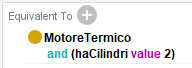
\includegraphics[scale=1]{img/spec_bicilindrico.png}
       \caption{Modellazione motore bicilindrico.} 
    \end{center}
\end{figure}
  \item \textbf{MotoreQuadricilindrico}: Rappresenta un motore dotato di quattro cilindri (che possono essere disposti seguendo diverse configurazioni).
    \begin{figure}[H]
    \begin{center}
        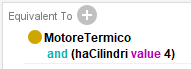
\includegraphics[scale=1]{img/spec_quadricilindrico.png}
       \caption{Modellazione motore quadricilindrico.} 
    \end{center}
\end{figure}
  \item \textbf{Posizionamento}: Rappresenta il risultato ottenuto dai partecipanti ad una gara (va a formare la classifica).
  \item \textbf{PosizionamentoCampionato}: Rappresenta il risultato ottenuto dai partecipanti al campionato (ottenuto applicando particolari criteri ai risultati delle singole gare e delle qualifiche).
  \item \textbf{PosizionamentoGara}: Rappresenta il posizionamento in una gara.
  \item \textbf{PosizionamentoQualifiche}: Rappresenta il risultato ottenuto dai partecipanti ad una sessione di qualifica.
  \item \textbf{Sponsor}: Rappresenta un'azienda, che fornisce supporto finanziario a una squadra o a un evento.
  \item \textbf{Team}: Rappresenta un team, che è composto da individui che competono insieme nel motomondiale.
  \item \textbf{Person}: Rappresenta un individuo.
  \item \textbf{Pilota}: Rappresenta l'individuo che conduce la moto in una gara motociclistica.
  \item \textbf{Leggenda}: Rappresenta un pilota che ha vinto almeno un campionato in ognuna delle tre categorie principali (Moto2, Moto3 e MotoGP), es. Valentino Rossi.
  \item \textbf{Staff}: Rappresenta membri dello staff coinvolti nel motomondiale.
  \item \textbf{Stuart}: Rappresenta un membro dello staff che lavora per uno specifico circuito.
    \begin{figure}[H]
    \begin{center}
        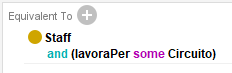
\includegraphics[scale=1]{img/spec_stuart.png}
       \caption{Modellazione stuart.} 
    \end{center}
\end{figure}
  \item \textbf{TeamStaff}: Rappresenta membri dello staff che lavorano per un team.
  \item \textbf{TeamManager}: Rappresenta un team manager, che è responsabile della gestione del team.
  \item \textbf{Capotecnico}: Individuo responsabile della gestione del team di meccanici e fautore delle decisioni tecniche.
    \begin{figure}[H]
    \begin{center}
        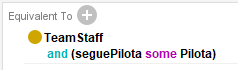
\includegraphics[scale=1]{img/spec_capotecnico.png}
       \caption{Modellazione capotecnico.} 
    \end{center}
\end{figure}
\end{itemize}

\subsection{Proprietà}
Le object properties rappresentano relazioni tra oggetti all'interno di uno dominio specifico. Nel nostro caso consentono di definire connessioni utili al processo di reasoning per inferire nuove informazioni ed utili all'ottenimento di statistiche composite per ognuna delle diverse entità che compongono Motology. 
Nella seguente sezione, vengono presentate proprietà utilizzate nel sistema, coadiuvate di una breve spiegazione per ciascuna di esse.

\begin{itemize}
    \item \textbf{guidaMoto}: Indica che un pilota guida una moto.
    \item \textbf{haCapotecnico}: Indica che un pilota fa riferimento ad un capo tecnico.
    
\item \textbf{haCircuito}: Indica che un soggetto ha un circuito associato.
    \item \textbf{ospitaCircuito}: Indica che una città ospita un circuito.
    \item \textbf{sponsorizzaCircuito}: Indica che uno sponsor (anche eventualmente un costruttore) finanzia un circuito ottenendo indietro pubblicità.
    \item \textbf{svoltoPresso}: Indica che un gran premio si svolge presso un circuito, questa proprità ne presuppone altre in quanto ogni nazione vede lo svolgersi di un gran premio in un solo circuito.
	
	\item \textbf{haCittà}: Indica che un soggetto è nato o situato in una specifica città.
    \item \textbf{natoInCittà}: Indica che un individuo è nato in una specifica città.
    \item \textbf{situatoInCittà}: Indica che un circuito è situato in una città.
	
	
    \item \textbf{haCostruttore}: Indica che un soggetto ha un costruttore, cioè un brand che produce prototipi di motociclette da competizione, associato.
    \item \textbf{costruitaDa}: Indica che una moto è costruita da un costruttore.
    \item \textbf{haCostruttoreDelTeam}: Indica che un team utilizza moto di un unico costruttore.
    \item \textbf{posizionamentoDiCostruttore}: Indica il posizionamento suddiviso in costruttori, applicando delle regole ai posizionamenti dei singoli piloti che utilizzano moto da tale costruttore.
	
    \item \textbf{haGP}: Indica che un campionato o una competizione hanno un gran premio associato.
    \item \textbf{compostoDaGP}: Indica che un campionato è composto da gran premi.
    \item \textbf{corsaInGP}: Indica che una competizione si svolge in un gran premio.
    \item \textbf{ospitaGP}: Indica che un circuito ospita un gran premio.
    \item \textbf{proveInGP}: Indica che un turno di prove libere si svolge in un gran premio.
	
    \item \textbf{haInClassifica}: Indica che una competizione ha un piazzamento in classifica.
    \item \textbf{haInScuderia}: Indica che un team ha una moto nella propria scuderia.
    \item \textbf{haMotore}: Indica che una moto ha un motore associato.
    \item \textbf{haNazione}: Indica che un oggetto proviene da o è associato ad una nazione.
      \begin{figure}[H]
    \begin{center}
        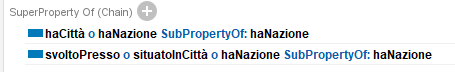
\includegraphics[scale=1]{img/spec_haNazione.png}
       \caption{Modellazione nazione.} 
    \end{center}
\end{figure}
    \item \textbf{haOttenuto}: Indica che un pilota ha ottenuto un piazzamento.
	
    \item \textbf{haPilota}: Indica che un oggetto è associato ad un pilota.
    \item \textbf{cittàNataleDi}: Indica la città natale di un pilota.
    \item \textbf{guidataDa}: Indica che una moto è guidata da un pilota.
    \item \textbf{piazzamentoDi}: Indica che un piazzamento è stato ottenuto da un pilota.
    \item \textbf{seguePilota}: Indica che un capo tecnico segue un pilota.
    \item \textbf{teamDi}: Indica che un team ha un pilota a contratto.
    \item \textbf{tempoDi}: Indica che un tempo è stato segnato da un pilota.
	
    \item \textbf{haSponsor}: Indica che un team o un circuito è associato ad uno sponsor.
    \item \textbf{teamSponsorizzatoDa}: Indica che un team è sponsorizzato da uno sponsor.
    \item \textbf{circuitoSponsorizzatoDa}: Indica che un circuito è sponsorizzato da uno sponsor.
	
    \item \textbf{haStaff}: Indica che un team ha uno staff.
	
    \item \textbf{haTeam}: Indica che ad un soggetto è associato un team.
    \item \textbf{dipendenteDelTeam}: Indica che un membro dello staff dipende da un team.
    \item \textbf{motoDelTeam}: Indica che una moto appartiene ad un team.
    \item \textbf{pilotaDelTeam}: Indica che un pilota corre per un team.
    \item \textbf{sponsorizzaTeam}: Indica che uno sponsor sponsorizza un team.
	
    \item \textbf{inClassificaDi}: Indica che il piazzamento concorre alla classifica di una competizione.
    \item \textbf{lavoraPer}: Indica che uno stuart lavora per un circuito.
    \item \textbf{montatoDa}: Indica che un motore è montato su una moto.
    \item \textbf{produttoreDi}: Indica che un produttore ha costruito una moto (non necessariamente il relativo motore).
    \item \textbf{qualificatoConTempo}: Indica che un posizionamento in qualifica ha un tempo associato.
    \item \textbf{svoltoInCampionato}: Indica che un gran premio è associato ad un campionato.
    \item \textbf{tempoInFP}: Indica che un tempo è associato ad una prova libera.
    \item \textbf{tempoInQ}: Indica che un tempo è associato ad un posizionamento in qualifica.
\end{itemize}

\subsection{Data Properties}
Le data properties consentono di specificare attributi e caratteristiche dei concetti rappresentati dalle classi della nostra ontologia. Di seguito, presentiamo un elenco delle data properties utilizzate da Motology, fornendo una breve spiegazione per ciascuna di esse.\\

\begin{itemize}
\item \textbf{haAnno}: Indica in che anno si svolge un campionato o un gran premio.
\item \textbf{haCilindrata}: Indica la cilindrata di un motore termico.
\item \textbf{haCilindri}: Indica il numero di cilindri di un motore termico.
\item \textbf{haCoppia}: Indica la coppia di un motore.
\item \textbf{haGap}: Indica il gap dal vincitore della gara.
\item \textbf{haLunghezza}: Indica la lunghezza di un circuito.
\item \textbf{haNome}: Indica il nome di un oggetto.
\item \textbf{haNomePersona}: Indica il nome proprio di una persona.
\item \textbf{haNumero}: Indica il numero di un pilota e della sua moto.
\item \textbf{haPosizioneFinale}: Indica la posizione del piazzamento in una competizione.
\item \textbf{haPotenza}: Indica la potenza di un motore.
\item \textbf{haPunti}: Indica i punti ottenuti dal piazzamento in classifica.
\item \textbf{haTempo}: Indica il miglior tempo registrato in una competizione o in un turno di prove.
\item \textbf{haTracciato}: Indica il collegamento all'immagine del tracciato.
\end{itemize}

\section{Regole SWRL}

Di seguito enunceremo le regole implementate in SWRL, per permettere al sistema di derivare informazioni dai dati che già possiede.

\begin{itemize}
  \item \textbf{Regola dello stesso anno}:\\
  
  La regola implica che se un gran premio si svolge in un campionato allora l'anno del GP sarà lo stesso del campionato.\\

  \texttt{moto:svoltoInCampionato(?gp, ?c) \textasciicircum\ moto:haAnno(?c, ?a)\\-> moto:haAnno(?gp, ?a)}

  \item \textbf{Regola del costruttore}:\\
  
  La regola implica che se un team ha degli accordi con uno specifico costruttore allora tutte le moto che ha in scuderia proverranno dallo stesso costruttore.\\

  \texttt{moto:haCostruttoreDelTeam(?t, ?c) \textasciicircum\ moto:haInScuderia(?t, ?m)\\-> moto:costruitaDa(?m, ?c)}

  \item \textbf{Regola del numero}:\\
  
  La regola implica che la moto guidata da un pilota, il quale sceglie il proprio numero, sarà associata al medesimo numero.\\

  \texttt{moto:guidataDa(?m, ?p) \textasciicircum\ moto:haNumero(?p, ?n)\\-> moto:haNumero(?m, ?n)}

  \item \textbf{Regola dello stesso team}:\\
  
  La regola implica che se un pilota fa parte di un team, allora anche la moto che guida rientrerà nella stessa scuderia.\\

  \texttt{moto:pilotaDelTeam(?p, ?t) \textasciicircum\ moto:guidaMoto(?p, ?m)\\-> moto:motoDelTeam(?m, ?t)}

  \item \textbf{Regola del capotecnico}:\\
  
  La regola implica che il capotecnico che segue un pilota apperterrà allo stesso team per il quale gareggia il pilota stesso.\\

  \texttt{moto:pilotaDelTeam(?p, ?t) \textasciicircum\ moto:haCapotecnico(?p, ?c)\\-> moto:dipendenteDelTeam(?c, ?t)}

  \item \textbf{Regola del tempo di piazzamento}:\\
  
  La regola implica che il miglior tempo registrato per il piazzamento in qualifica di un pilota sia stato registrato dal pilota stesso.\\

  \texttt{moto:piazzamentoDi(?piaz, ?pil) \textasciicircum\ moto:qualificatoConTempo(?piaz, ?t)\\-> moto:tempoDi(?t, ?pil)}

  \item \textbf{Regola della leggenda}:\\
  
  La regola implica che se un pilota risulta aver vinto almeno una volta ciascuno dei tre attuali campionati principali, Moto3, Moto2 e MotoGP, allora potrà essere annoverato tra le leggende.\\

  \texttt{moto:Pilota(?p) \textasciicircum\\ moto:haOttenuto(?p, ?piazz1) \textasciicircum\ moto:inClassificaDi(?piazz1, ?ch1) \textasciicircum\ moto:Moto3(?ch1) \textasciicircum\ moto:haPosizioneFinale(?piazz1, 1) \textasciicircum\\ moto:haOttenuto(?p, ?piazz2) \textasciicircum\ moto:inClassificaDi(?piazz2, ?ch2) \textasciicircum\ moto:Moto2(?ch2) \textasciicircum\ moto:haPosizioneFinale(?piazz2, 1) \textasciicircum\\ moto:haOttenuto(?p, ?piazz3) \textasciicircum\ moto:inClassificaDi(?piazz3, ?ch3) \textasciicircum\ moto:MotoGP(?ch3) \textasciicircum\ moto:haPosizioneFinale(?piazz3, 1)\\-> moto:Leggenda(?p)}

\end{itemize}